% Klassifiziert den Dokumenten-Typ
% Doku: http://exp1.fkp.physik.tu-darmstadt.de/tuddesign/
% Farben: http://www.tu-darmstadt.de/media/medien_stabsstelle_km/services/medien_cd/das_bild_der_tu_darmstadt.pdf
%  bigchapter: Chapter haben doppelte Schriftgröße
%  linedtoc: Linien im Inhaltsverzeichnis wie bei Überschriften
%  colorbacktitle: Der Dokumenten-Titel wird mir der Accentfarbe hinterlegt
\documentclass[bigchapter,colorback,accentcolor=tud4b,linedtoc,11pt]{tudreport}

% Input Dokument hat das Encoding UTF-8
\usepackage[utf8]{inputenc}
% Wichtiges Paket für Links und verlinktes Inhaltsverzeichnis
\usepackage[ngerman]{hyperref}
% Paket für Fußnoten
\usepackage[stable]{footmisc}
\usepackage{multirow}
% Alternatives package für bilder
\usepackage{wrapfig}
% Paket für amsmath (aligned mathe formeln)
\usepackage{amsmath}
% Farbige tabellen
\usepackage{colortbl}


% Paket für Bibliotheks-Verzeichnis, square: Verwende eckige statt runde klammern
% \usepackage[square]{natbib}
% Paket zum Plotten von Datensätzen
\usepackage{pgfplots}
\pgfkeys{%
  /pgfplots/default/.style={%
    /pgf/number format/use comma,
    legend pos=north east,
    x tick label style={/pgf/number format/1000 sep=},
    y tick label style={/pgf/number format/1000 sep=},
    width=0.9\linewidth,
    height=0.40\linewidth,
    scale only axis,
    grid=both,
    tick align=outside,
    tickpos=minor,
    left X tick num=3,
    minor y tick num=4,
    minor grid style={dotted,thin}
  }
}

% Anhänge für Original-Messdaten
\usepackage{fancyvrb}

% Verwende deutsche Bezeichner für Inhaltsverzeichnis, ... (ngerman = New German: neue Rechtschreibung)
\usepackage{ngerman}
% Deutsche Zahlen (entfernt z.B. das Leerzeichen nach einem Dezimal-Komma)
\usepackage{ziffer} 

\usepackage[verbose]{placeins}

%wegen Grafikverschiebung hinzugefügt
\usepackage{float}

%\usepackage{graphicx}
%\usepackage{caption}
\usepackage{subcaption} %Für subfigures

% PDF-Optionen
\hypersetup{%
  pdftitle={TU Darmstadt \- Physikalisches Praktikum für Fortgeschrittene},
  pdfauthor={Esra Bauer, Sören Link und Christian Hab},
  pdfsubject={Versuch 1.5},
  pdfview=FitH,
}
% Nummeriere formeln in Subsections einzeln
% Kleines makro zur assymetrischen Fehlerangabe

% Entspricht-Zeichen
\usepackage{scalerel}

\newcommand\equalhat{%
\let\savearraystretch\arraystretch
\renewcommand\arraystretch{0.3}
\begin{array}{c}
\stretchto{
    \scalerel*[\widthof{=}]{\wedge}
    {\rule{1ex}{3ex}}%
}{0.5ex}\\ 
=%
\end{array}
\let\arraystretch\savearraystretch
}
%BEGINN TITELSEITE

\title{Zeeman-Effekt}

\subtitle{Esra Bauer  \\Sören Link \\Christian Hoch}

\subsubtitle{Betreuer: Matthias Sattig \hfill Versuchsdatum: 13. April 2015}

\author{Esra Bauer, Sören Link, Christian Hoch}

%\settitlepicture{img/title.jpg}

\institution{Physikalisches Praktikum \\für Fortgeschrittene \\ Versuch 1.5}

\date{\today}
%ENDE TITELSEITE


\begin{document}
%ANFANG DOKUMENT

%Titelseite einfügen
\maketitle

%Inhaltsverzeichnis einfügen
\tableofcontents

%ANFANG INHALT
\chapter{Einleitung}


\chapter{Grundlagen}


\section{Fabry-Pérot-Interferometer}

\begin{figure}[H] 
  \centering
     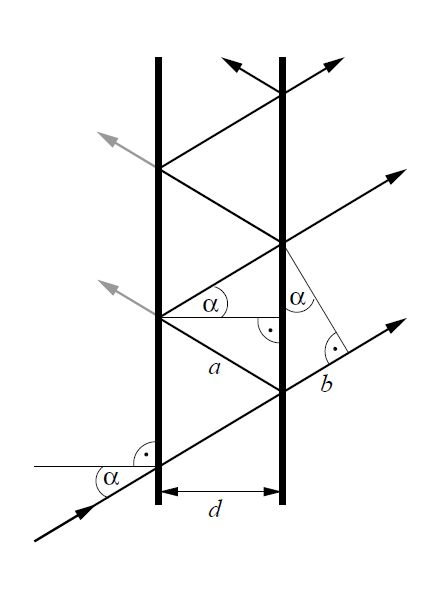
\includegraphics[width=0.4\textwidth]{data/Fabry.jpg}
  \caption{Strahlengang im Fabry-Pérot-Interferometer.}
  \label{fig:Bild1}
\end{figure}

Das Fabry-Pérot-Interferometer wird in diesem Versuch genutzt, um
Aussagen über die Frequenz von elektromagnetischer Strahlung zu machen.
Es besteht aus zwei parallelen Spiegeln mit hoher Reflektivität, welche
im Abstand $d$ zu einander angeordnet sind. Im Zwischenraum befindet
sich Luft. \\
Betrachtet man einen einfallenden Lichtstrahl im Winkel $\alpha$ zur
Spiegelnormalen, so wird ein Teil davon durch beide Spiegel transmittiert,
wohingegen ein anderer Teil einmal an beiden Spiegeln reflektiert
und dann erst durch den zweiten Spiegel hindurchgelassen wird. Obwohl
es auch noch Strahlen gibt, die viel öfter zwischen den Spiegeln hin
und her reflektiert werden, betrachten wir erst einmal diese beiden
Teilstrahlen. Nach dem Austritt aus dem zweiten Spiegel haben sie
einen Gangunterschied von $s=2a-b=2dcos\alpha$. Ist $s=n\lambda$,
also ein ganzzahliges Vielfaches der Wellenlänge, so tritt konstruktive
Interferenz auf. \\
Sei $\delta\alpha_{2}$ der Winkel zwischen zwei Interferenzordnungen,
$\delta\alpha_{1}$ der Winkel zwischen zwei Spektrallinien der selben
Interferenzordnung und $\triangle g_{eff}$ die $g_{eff}$-Differenz
zwischen selbigen, so ergibt sich in der Nähe der höchsten Interferenzordnung
folgender Zusammenhang mit dem Bohrschen Magneton:

$$\mu_{B}=\frac{hc}{2dB}\frac{\delta\alpha_{1}}{\triangle g_{eff}\delta\alpha_{2}}$$

Messtechnisch gibt man nun $\delta\alpha$ in Einheiten von $g_{eff}$
an. Somit kürzt sich $\triangle g_{eff}$ und $\delta\alpha_{1}$
heraus und man muss nur noch $\delta\alpha_{2}$ bestimmen. Das geht
am einfachsten, wenn man das Magnetfeld so einstellt, dass sich die
energetisch höchste/niedrigste Linie mit der niedrigsten/höchsten
Linie der eins niedrigeren/höheren Ordnung überlappt. Denn genau dann
gilt $\delta\alpha_{2}=$ $2g_{eff,MAX}$, wobei $g_{eff,MAX}$ das
größtmögliche $g_{eff}$ eines Übergangs ist. 


\section{Klassische Erklärung des Zeeman-Effekts}

\begin{figure}[H] 
  \centering
     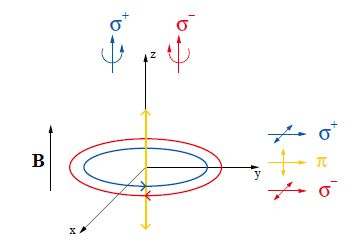
\includegraphics[width=0.6\textwidth]{data/Zerlegung.jpg}
  \caption{Veränderung der Ionenoszillation durch ein äußeres Magnetfeld.}
  \label{fig:Bild1}
\end{figure}


Nach der klassischen Theorie ist für die Emission eines Lichtquants
die Oszillation eines geladenen Teilchens, eines Ions, verantwortlich.
Wird zusätzlich dazu ein Magnetfeld angelegt (in z-Richtung), so wirkt
auf das Ion die Lorentzkraft und es beginnt, mit der Lamorfrequenz
$\omega_{L}$ um die z-Achse zu präzedieren. Während die z-Komponente
der Oszillation des Ions unverändert bleibt, kommt es bei den Komponenten
senkrecht zum Magnetfeld zu einer Kreisbewegung um die z-Achse, dessen
Frequenz um $\omega_{L}$ einmal abgeschwächt und rechtsdrehend um
die z-Achse und ein anderes mal verstärkt und linksdrehend zu beobachten
ist. \\
Man kann sich die Lichtemission nun vorstellen, wie einen Hertzschen
Dipol, wobei das Ion die bewegte Ladung darstellt und der Dipol nur
senkrecht zu dieser Bewegungsrichtung abstrahlt. \\
Schaut man nun also transversal zum Magnetfeld auf das Teilchen, so
wird man in Magnetfeldrichtung ($\pi$-Komponente) die vom Magnetfeld
unabhängige emittierte Frequenz $\omega$ beobachten, senkrecht dazu
jedoch die je um $\omega_{L}$ nach unten bzw. nach oben verschobenen
Frequenzen der $\sigma^{-/+}$-Komponenten. In diesem Fall sind alle
Komponenten linear polarisiert. \\
Schaut man longitudinal zum Magnetfeld, sieht man nur die $\sigma^{-/+}$-Komponenten,
welche jeweils zirkular polarisiert sind. 


\section{Quantenmechanische Kopplungen im Atom}

Betrachtet man ein Atom, wo wird es quantenmechanisch durch den Hamiltonoperator
beschrieben:

$$\hat{H}=\hat{T}+\hat{V}_{C}+\hat{V}_{ss}+\hat{V}_{ll}+\hat{V}_{ls}$$

Er setzt sich zusammen aus $\hat{T}$, dem Operator der kinetischen
Energie, $\hat{V}_{C}$, der Coulomb-Wechselwirkung und den magnetischen
Wechselwirkungen $\hat{V}_{ss},\mbox{ }\hat{V}_{ll}\mbox{ und }\hat{V}_{ls}$.


\subsection{LS-Kopplung}

Ist $\hat{V}_{ls}$ viel kleiner als die beiden anderen mag. Wechselwirkungen,
so koppeln die einzelnen Elektronenspins zu einem Gesamtspin $S=\sum s_{i}$
und genauso die Elektronendrehimpulse zu einem Gesamtbahndrehimpuls
$L=\sum l_{i}$. Diese koppeln dann zu einem Gesamtdrehimpuls $J=\left|L-S\right|,\mbox{ }\left|L-S\right|+1,\mbox{ ... }\left|L+S\right|$.\\
Es ist üblich, den Zustand eines Atoms in der Notation nach Russel
und Saunders anzugeben:

$$^{(2S+1)}L_{J}$$



\subsection{jj-Kopplung}

Hier ist $\hat{V}_{ls}$ deutlich größer als die beiden anderen mag.
Wechselwirkungen. Es koppeln Spin und Bahndrehimpuls eines Elektrons
zu einem Gesamtdrehimpuls $j_{i}=l_{i}+s_{i}$ eines Elektrons. Diese
koppeln dann zu einem Gesamtdrehimpuls des Atoms $J=\sum j_{i}$.


\section{Quantenmechanische Erklärungen}

Legt man ein Magnetfeld (in z-Richtung) an, so ergänzt sich der Hamiltonoperator
eines Atoms um die magnetische Störung $\hat{H}_{B}=-\hat{\mu}\vec{B}$
mit $\hat{\mu}=\underset{i}{\sum}(\hat{\mu}_{l_{i}}+\hat{\mu}_{s_{i}})=\underset{}{\frac{\mu_{B}}{\hslash}\underset{i}{\sum}(g_{L}\hat{l}_{i}+g_{S}\hat{s}_{i})}$,
wobei für die Landéschen g-Faktoren gilt: $g_{L}=1$ und $g_{S}\thickapprox2$. 


\subsection{Quantenmechanische Erklärung des Zeeman-Effekts}

Beim Zeeman-Effekt ist das Magnetfeld klein im Vergleich zu den Wechselwirkungen
im Atom. Das heißt, es kommt zur LS-Koppelung und der Hamiltonoperator
der magnetischen Störung nimmt die Form $\hat{H}_{Ze}=\frac{\mu_{B}}{\hslash}g_{J}\hat{J}\vec{B}$
an. Die Eigenwerte dieses Operators geben die Zeeman-Energien: $E_{Ze}=\mu_{B}Bg_{J}M_{J}$.
Dabei ist $M_{J}$ die magnetische Quantenzahl. Für $g_{J}$ ergibt
sich: $g_{J}=g_{L}+(g_{S}-g_{L})\frac{J(J+1)-L(L+1)+S(S+1)}{2J(J+1)}$.
Für den Übergang von einem Niveau $a$ zum Niveau $a'$ ergibt sich
somit eine Energiedifferenz von $\triangle E_{Ze}$: $\frac{\triangle E_{Ze}}{\mu_{B}B}=(g_{J}M_{J}-g_{J}'M_{J}')=g_{eff}$\\
Betrachtet man einen Übergang von $S=0$ nach $S=0$, so handelt es
sich um den normalen Zeeman-Effekt. Bei diesem vereinfacht sich $g_{eff}$
zu $g_{L}\triangle M_{L}$.\\
Vergleicht man nun mit der klassischen Erklärung, so entspricht die
$\pi$-Komponente einem Übergang mit $\triangle M=0$ und die $\sigma^{+/-}$-Komponente
einem Übergang mit $\triangle M=\pm1$. Das gilt auch für den nachfolgenden
Paschen-Back-Effekt.


\subsection{Quantenmechanische Erklärung des Paschen-Back-Effekts}
>>>>>>> origin/master

Beim Paschen-Back-Effekt ist das angelegte Magnetfeld so groß, dass
die Spin-Bahn-Wechselwirkung aufgehoben wird. Somit sind Gesamtspin
und Gesamtbahndrehimpuls entkoppelt. Es kann sein, dass diese Entkopplung
bei noch nicht so starkem Magnetfeld zunächst nur eines der am Übergang
beteiligten Energieniveaus betrifft. Dann spricht man vom partiellen
Paschen-Back-Effekt; andererseits vom vollständigen. Im Fall von Entkopplung
gilt: $\hat{H}_{PB}=\frac{\mu_{B}}{\hslash}(g_{L}\hat{L}+g_{S}\hat{S})\vec{B}$
und somit $E_{PB}=\mu_{B}B(g_{L}M_{L}+g_{S}M_{S})$.\\
Im Falle des vollständigen Paschen-Back-Effekts kommt es zum selben
$g_{eff}$, wie beim normalen Zeeman-Effekt (da $\triangle M_{S}=0$,
siehe Auswahlregeln) und somit sind diese beiden Effekte aus spektroskopischer
Sicht ununterscheidbar. 


\section{Auswahlregeln für Dipolübergänge}

Sind Gesamtbahndrehimpuls und Gesamtspin zum Gesamtdrehimpuls gekoppelt,
wie beim Zeeman-Effekt, so gelten folgende Auswahlregeln:
\begin{itemize}
\item $\triangle J=0,\mbox{ }\pm1$
\item $\triangle M_{J}=0$ (außer $\triangle J=\text{0}$), $\pm1$
\end{itemize}
Sind Gesamtbahndrehimpuls und Gesamtspin entkoppelt, wie beim Paschen-Back-Effekt,
so gelten folgende Auswahlregen:
\begin{itemize}
\item $\triangle L=0,\mbox{ }\pm1$
\item $\triangle M_{L}=0,\mbox{ }\pm1$
\item $\triangle M_{S}=0$\end{itemize}

\chapter{Durchführung}
\section{Messung von $\frac{\delta\alpha_1}{\Delta g_{eff} \delta\alpha_2}$}

Um das Bohrsche Magneton zu berechnen, benötigen wir neben dem verwendeten
Magnetfeld, welches wir mit Hilfe einer Hall-sonde bestimmen, noch das
Verhältniss von $\delta\alpha_1$ zu $\Delta g_{eff} \delta\alpha_2$.

Um dieses verhältniss bestimmen zu können, müssen zunächst mit Hilfe eines
Farbfilters die sichtbaren Spektrallinien reduziert werden. Dazu stehen uns Filter
mit Wellenlängen von $405 nm \pm 1\%$, $436 nm \pm 1\%$ und $546 nm \pm 1\%$
zur verfügung, welche bei der verwendeten Quecksilberdampflampe den Übergängen von
$2^3S_1$ nach $2^3P_0$, $2^3P_1$ und $2^3P_2$ entprechen. Durch das angelegte
Magnetfeld wird die Entartung der Energieniveaus entsprechend des anormalen
Zeeman-Effekts aufgehoben und wir können mit Hilfe der an das
Fabrey-Perot-Interferometer angeschlossenen Kamera mehrere
Spektrallinien beobachten.

Durch veränderung der Magnetfeldstärke lassen sich die im Interferometer
beobachteten Spektrallinien weiter verschieben. Zur Messung von
$\frac{\delta\alpha_1}{\Delta g_{eff} \delta\alpha_2}$ wird das Magnetfeld so
eingestellt, dass sich Spektrallinien von benachtbarten Interferenzordnungen
überlagern. 

\begin{figure}[H] 
  \centering
     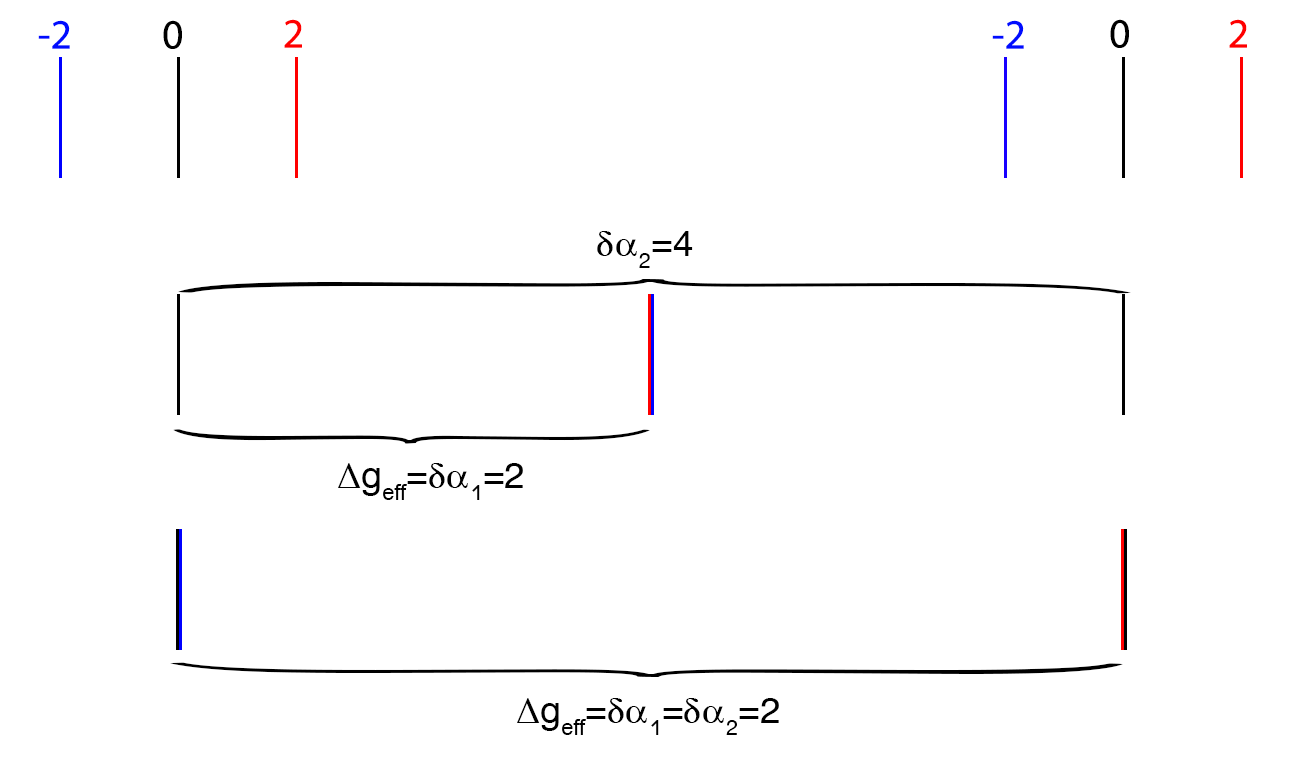
\includegraphics[width=0.8\textwidth]{img/linienspektrum405.png}
  \caption{Linienspektrum bei Verwendung des 405nm Filters. Beide gezeigten
    Einstellungen wurden für die Messung verwendet.}
  \label{fig:405nmlines}
\end{figure}

\begin{figure}[H] 
  \centering
     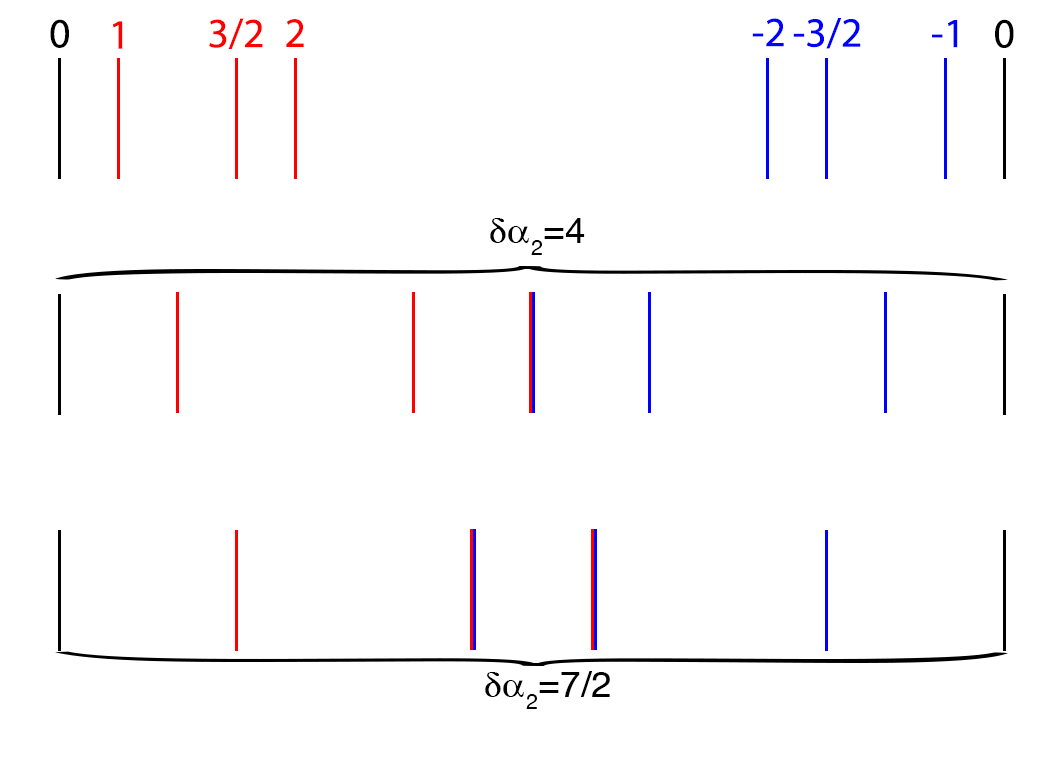
\includegraphics[width=0.8\textwidth]{img/linienspektrum436.png}
     \caption{Linienspektrum bei Verwendung des 436nm Filters. Da die einzelnen
       Spektrallinien bei der oberen Einstellung nicht klar voneinander zu
       unterscheiden waren, wurde für die Messung lediglich die untere
       Eisntellung verwendet.}
  \label{fig:436nmlines}
\end{figure}

\begin{figure}[H] 
  \centering
     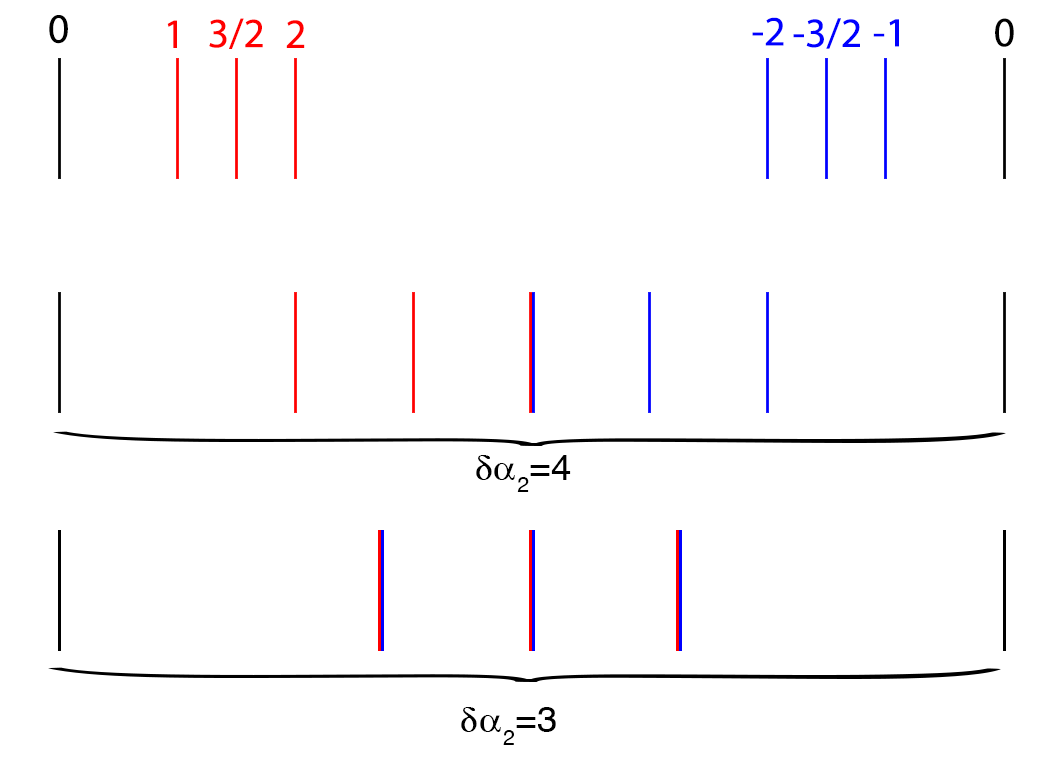
\includegraphics[width=0.8\textwidth]{img/linienspektrum546.png}
     \caption{Linienspektrum bei Verwendung des 546nm Filters. Auch hier wurde
       lediglich die unterste Einstellung für die Messungen verwendet, da die
       einzelnen Spektrallinien sonst nicht eindeutig genug zu unterscheiden waren.}
  \label{fig:546nmlines}
\end{figure}


\begin{center}
  \begin{tabular}{|c|c|c|c|}
    \hline
    \multirow{2}{*}{Messung} & \multicolumn{3}{c|}{B in Tesla}     \\ \cline{2-4}
                             & 405nm Filter & 436nm Filter & 546nm Filter
                                                                   \\ \hline 
    1                        & 0,362        & 0,400        & 0,472 \\ \hline
    2                        & 0,726        & 0,399        & 0,484 \\ \hline
    3                        & 0,391        & 0,403        & 0,488 \\ \hline
    4                        & 0,723        & 0,390        & 0,480 \\ \hline
    5                        & 0,365        & 0,396        & 0,490 \\ \hline
    6                        & 0,741        & 0,393        & 0,485 \\ \hline
    7                        & 0,366        & 0,393        & 0,499 \\ \hline
    8                        & 0,730        & 0,393        & 0,480 \\ \hline
    9                        & 0,377        & 0,392        & 0,489 \\ \hline
    10                       & 0,733        & 0,393        & 0,487 \\ \hline
	\end{tabular}
     \caption{Linienspektrum bei Verwendung des 546nm Filters. Auch hier wurde
       lediglich die unterste Einstellung für die Messungen verwendet, da die
       einzelnen Spektrallinien sonst nicht eindeutig genug zu unterscheiden waren.}
\end{center}

Da unser Versuchsaufbau eine genaue Fehlerabschätzung nahezu unmöglich macht,
wurden für jeden verwendeten Filter 10 Messungen durchgeführt. Der von uns
errechnete Wert für das Bohrsche Magneton bestimmt sich dann aus dem Mittelwert
und der Standardabweichung der aufgenommenen Messdaten.

Um den Einfluss von systematischen Fehlern beim Einstellen des Magnetfeldes auf
die Messungen zu reduzieren, wurden für jeden der beobachteten Übergängen die
Messungen abwechselnd von allen 3 Prektikumsteilnehmern durchgeführt.


% \begin{tabular}{p{0cm} p{2cm} p{0cm}}
%  0 &  & 2  \\
%  \multicolumn{1}{p{0cm}|}{} &  &\multicolumn{1}{|p{0cm}}{}  \\
%  \multicolumn{3}{c}{\raisebox{1.5ex}{\smash{$\underbrace{\makebox[2cm]{}}_{\delta\alpha_1}$}}} \\
% \end{tabular}
% Am
% einfachsten lassen sich diese Werte in unserem Aufbau messen, indem man das
% angelegte Magnetfeld so einreguliert, dass sich die äußeren Niveaus zweier
% benachtbarter Interferenzringe überlagern. In diesem Fall ist $\delta\alpha_1$
% der Abstand eines nicht verschobenen übergangs zum äußersten sich mit dem
% nächsten Interferenzring überlagernden Übergangs. Da sich die Einheiten von
% $\delta\alpha_1$ und $\delta\alpha_1$ gegenseitig aufheben, kann man sie als
% vielfaches von $g_{eff]}$ schreiben. Dadurch lassen sich $\delta\alpha_1$ und
% $\Delta g_{eff}$ kürzen und als einzige Messgröße neben dem angelegten
% Magnetfeld verbleibt $\delta\alpha_2$.






\chapter{Auswertung}
\section{Überprüfung der Vorhersagen der klassischen Erklärung}

Zunächst betrachten wir den Fall des transversalen Zeeman-Effektes, also des senkrecht zur Blickrichtung ausgerichteten Magneten. In der Tat können wir, wenn der Linearpolarisator parallel zum Magnetfeld ausgerichtet ist, genau eine Spektrallinie beobachten, die bei geringfügiger Drehung des Linearpolarisators in beide Richtungen schwächer wird. Dies zeigt, dass lediglich parallel zum Magnetgeld polarisiertes Licht detektiert wird, was der Vorhersage des klassischen Modells entspricht. Wir sehen die $\pi$-Komponente, die in Richtung der z-Achse (also der Magnetfeldrichtung) schwingt und daher nicht vom Magnetfeld beeinflusst wird, also auch die gleiche Frequenz wie vorher besitzt.

Bei senkrecht zum Magnetfeld ausgerichtetem Linearpolarisator sehen wir zwei Spektrallinien im gleichen Abstand links und rechts der ursprünglichen Linie (bzw. links und rechts der $\pi$-Komponente). Daraus folgt, dass die Frequenzen dieser beiden Linien um einen bestimmten Betrag verschoben sind. Weiterhin werden die Linien schwächer, wenn man den Polarisator von der senkrechten Position wegdreht. Wir sehen hier die $\sigma^+$- und $\sigma^-$-Komponenten, die in Richtung der x-Achse schwingen, also senkrecht zum Magnetgeld polarisiert sind und um Frequenzen $\pm \omega$ von der ursprünglichen Linie abweichen.

Analog bestätigt sich das klassische Modell für den Fall des longitudinalen Zeeman-Effektes, bei dem mittels des $\frac{\lambda}{4}$-Plättchens, welches um 45$^{\circ}$ zum Linearpolarisator verdreht in den Strahlengang gebracht wird, nachgewiesen wird, dass lediglich zwei zirkular polarisierte Komponenten vorhanden sind, die entgegengesetzen Drehsinn besitzen und wiederum frequenzverschoben sind. Dies sind die $\sigma^+$- und $\sigma^-$-Komponenten, wobei die $\sigma^+$-Komponente einen mathematisch positiven Drehsinn besitzt. Dass die $\pi$-Komponente nicht sichtbar ist, erklärt sich dadurch, dass ein Hertzscher Dipol, als welchen wir das schwingende "`Ion"' betrachten, in Bewegungsrichtung nicht abstrahlt. Somit ist die klassische Vorhersage sowohl für den transversalen, als auch für den longitudinalen Zeeman-Effekt bestätigt.

\section{Überprüfung der Vorhersagen der quantenmechanischen Erklärung}

Um unsere Messdaten auswerten zu können, sind zunächst einige theoretische Vorüberlegungen notwendig. Als erstes berechnen wir die gyromagnetischen Faktoren der beteiligten Energieniveaus und tragen sie tabellarisch auf: 

\begin{center}
  \begin{tabular}{|p{2.2cm}|p{4cm}|p{2cm}|p{2cm}|}
    \hline
    Übergang & Wellenlänge in nm & $g_J$ & $g_J'$  \\ \hline
    $2^3S_1~\rightarrow~2^3P_0$ & 405 & 2 & - \\ \hline
    $2^3S_1~\rightarrow~2^3P_1$ & 436 & 2 & $\frac{3}{2}$ \\ \hline
    $2^3S_1~\rightarrow~2^3P_2$ & 546 & 2 & $\frac{3}{2}$ \\ \hline
	\end{tabular}
\end{center}

Zeichnerisch lassen sich die erlaubten Übergänge unter Berücksichtung der Auswahlregeln in folgenden Termschemata darstellen:

\begin{figure}[H] 
  \centering
     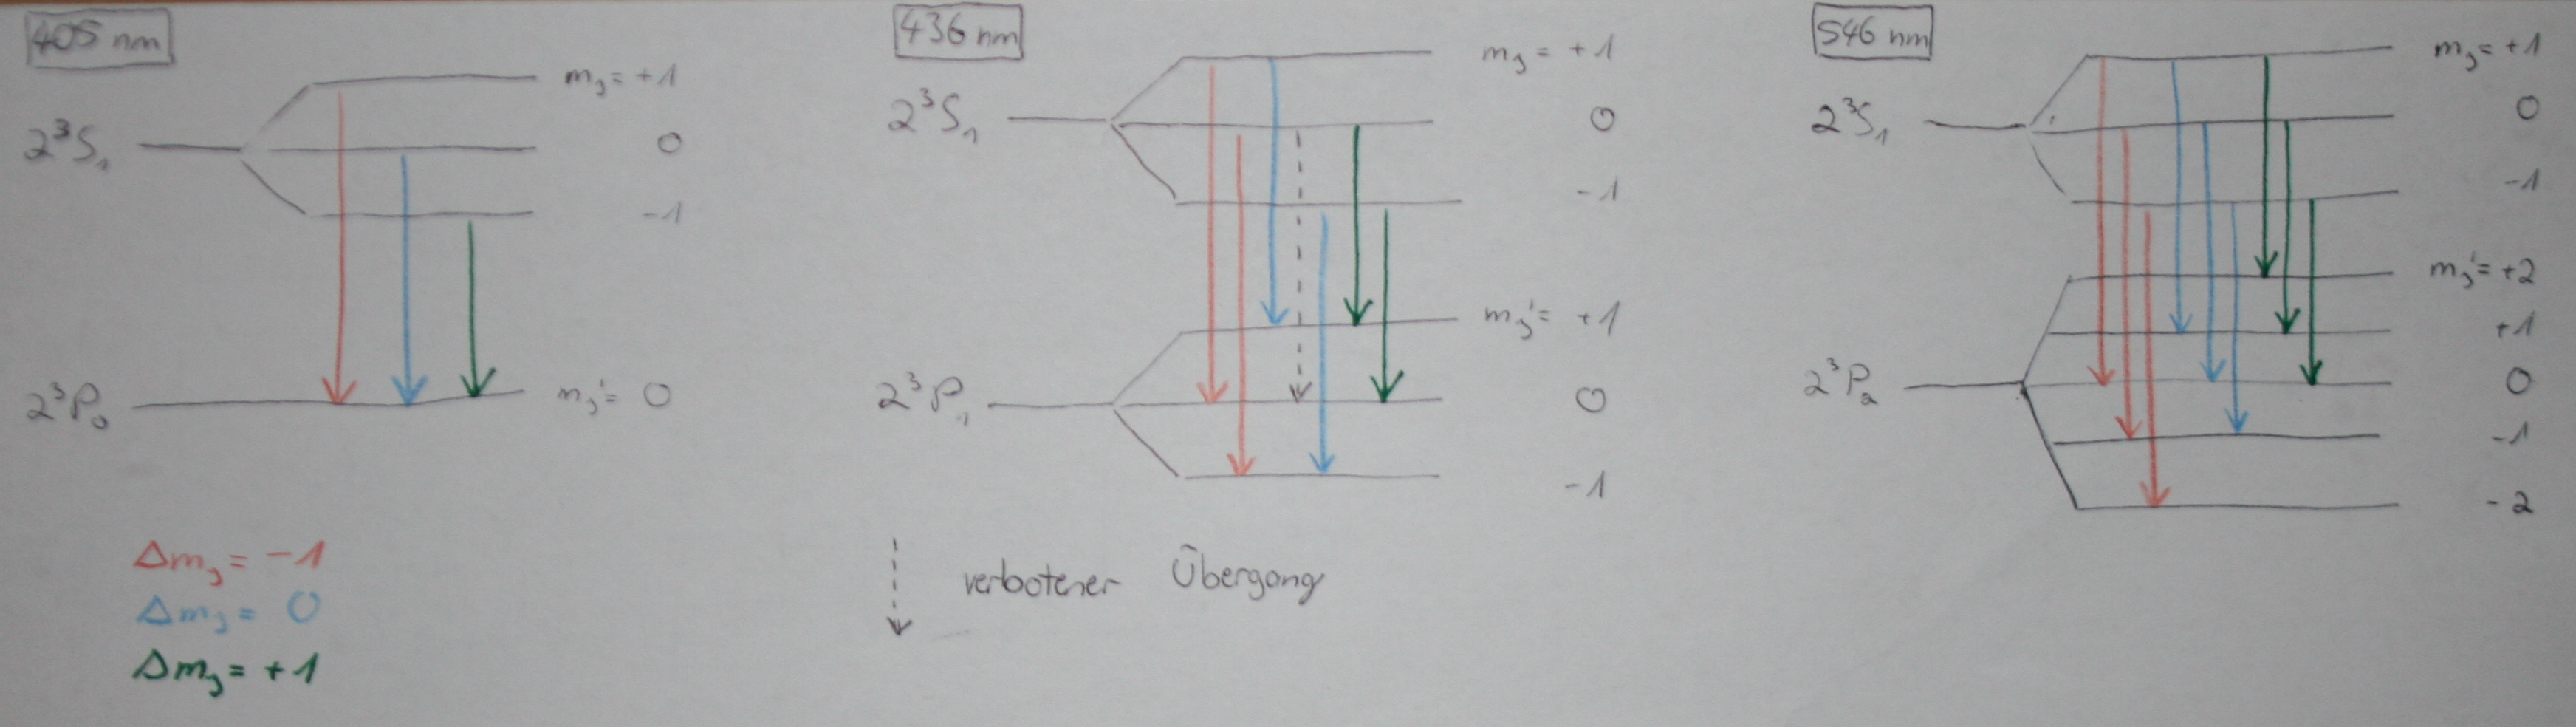
\includegraphics[width=1\textwidth]{data/Termschemata.JPG}
  \caption{Termschemata für alle drei Übergänge, oben sind jeweils die Wellenlängen eingeschrieben; verschiedene $\Delta m_J$ sind farblich gekennzeichnet. Verbotene Übergänge sind gestrichelt eingezeichnet.}
  \label{fig:Bild1}
\end{figure}

Die $g_{eff}$-Werte lassen sich leicht gemäß $g_{eff} = g_J M_J - g_J' M_J'$ berechnen und sind in folgenden Tabellen für jeden Übergang dargestellt, jeweils unterteilt in die möglichen Werte von $\Delta m_J$, also für die Änderung der magnetischen Gesamtdrehimpulsquantenzahl, die die möglichen Raumrichtungen des Drehimpulses angibt. Zunächst für 405 nm (hier ergeben sich drei Linien):

\begin{center}
  \begin{tabular}{|p{2cm}|p{2cm}|p{2cm}|p{2cm}|}
    \hline
    $\Delta m_J$ & $m_J$ & $m_J'$ & $g_{eff}$ \\ \hline
    1               & -1               & 0 & 2 \\ \hline
    0               & 0                & 0 & 0 \\ \hline
    -1              & 1                & 0 & -2 \\ \hline
	\end{tabular}
\end{center}

Für 436 nm sind es 6 Linien:

\begin{center}
  \begin{tabular}{|p{2cm}|p{2cm}|p{2cm}|p{2cm}|}
    \hline
    $\Delta m_J$ & $m_J$ & $m_J'$ & $g_{eff}$ \\ \hline
    1               & -1               & 0 & -2 \\ \hline
    1               & 0                & 1 & $-\frac{3}{2}$ \\ \hline
    0               & -1               & -1 & $-\frac{1}{2}$ \\ \hline
    0               & 1                & 1 & $\frac{1}{2}$ \\ \hline
   -1               & 0                & -1 & $\frac{3}{2}$ \\ \hline    
   -1               & 1                & 0 & 2 \\ \hline
    \end{tabular}
\end{center}

Für 546 nm ergeben sich sogar 9 Linien:

\begin{center}
  \begin{tabular}{|p{2cm}|p{2cm}|p{2cm}|p{2cm}|}
    \hline
    $\Delta m_J$ & $m_J$ & $m_J'$ & $g_{eff}$ \\ \hline
    1               & -1               & 0 & -2 \\ \hline
    1               & 0                & 1 & $-\frac{3}{2}$ \\ \hline
    1               & 1                & 2 & -1 \\ \hline
    0               & -1               & -1 & $-\frac{1}{2}$ \\ \hline
    0               & 0                & 0 & 0 \\ \hline
    0               & 1                & 1 & $\frac{1}{2}$ \\ \hline
    -1              & -1               & -2 & 1 \\ \hline
    -1              & 0                & -1 & $\frac{3}{2}$ \\ \hline
    -1              & 1                & 0 & 2 \\ \hline
    \end{tabular}
\end{center}

\section{Bestimmung des Bohrschen Magnetons}

Wie bereits vorher erklärt, berechnen wir das Bohrsche Magneton gemäß

$$\mu_{B}=\frac{hc}{2dB}\frac{\delta\alpha_{1}}{\triangle g_{eff}\delta\alpha_{2}}$$.

$\Delta \alpha_2$ ist für 405 nm 2 bzw. 4, da hier aufgrund der guten Ablesbarkeit zwei verschiedene Positionen gemessen werden konnten, für 436 nm beträgt der Wert $\frac{7}{2}$ und für 546 nm genau 3. Somit ergeben sich nach Mittelwertbildung folgende Werte:

\begin{center}
  \begin{tabular}{|p{2cm}|p{4cm}|p{2cm}|p{2cm}|}
    \hline
    Übergang & $< \mu_B >$ in $10^{-24}~ \frac{J}{T}$ & $\sigma_{\mu_B}$ & $\sigma_{\mu_B}$ in \% \\ \hline
    405               & 8,923 & 0,211 & 2,37  \\ \hline
    436               & 9,512 & 0,1 & 1,05  \\ \hline
    546               & 9,052 & 1,085 & 1,2  \\ \hline
    \end{tabular}
\end{center}

\chapter{Fazit}

Bei der qualitativen Überprüfung der klassischen Erklärung des Zeeman-Effektes treten keine Probleme auf bzw. mit den zur Verfügung stehenden Messintrumenten kann das Modell eindeutig bestätigt werden. Bei der Überprüfung des quantenmechanischen Modells muss quantitativ gearbeitet werden, um z.B. das Bohrsche Magneton zu berechnen. Hierbei fällt auf, dass für jeden Übergang eine mehr oder weniger große systematische Abweichung besteht. Betrachtet man den Mittelwert über alle Werte, ergibt sich jedoch eine gute Annäherung an den Literaturwert von $9,274 \cdot 10^{-24}~ \frac{J}{T}$. Dass bei nahezu jeder Messreihe eine systematische Abweichung besteht, liegt vermutlich in der ungenauen Ablesbarkeit begründet. Da das Bild der Kamera nur schwer zu erkennen ist bzw. die genaue Position der Überlappung kaum zu ermitteln ist, ergeben sich hierbei Fehler. Dennoch war die Berechnung des Bohrschen Magnetons bis auf eine relative Ungenauigkeit von etwa 0,1 möglich, was im Rahmen der Möglichkeiten als gutes Ergebnis anzusehen ist.

%ENDE INHALT
\cleardoublepage{}
% Eintrag fürs Inhaltsverzeichnis
\newpage
\begin{thebibliography}{100}
  \bibitem{Anleitung} \url{Versuchsanleitung}
\end{thebibliography}
\end{document}
